\documentclass[a4paper,12pt]{article}
\usepackage[utf8]{inputenc}
\usepackage[top=2.5cm, bottom=2.5cm, left=2.5cm, right=2.5cm]{geometry}
\usepackage[english]{babel}
\usepackage{graphicx}


% Title Page
\title{Université Libre de Bruxelles\\
INFO-F-404: Real-Time Operating Systems\\
2014 - 2015 Project 2: Game of life}
\author{Picard Simon}
\date{December 12, 2014}

\begin{document}
\maketitle
\clearpage
\tableofcontents
\clearpage

\section{Introduction}
The purpose of the project is to implement a "Game of life" simulator using several core at the same time.
 
\section{Choice of implementation}
The program should output a image, I choose the format pbm because it is really small. There is some headers including the width and the heigh of the image and then each 0 will be a white pixel and each 1 will be a black pixel.\\
I choose this format because the image generation process cannot be done by several process, so when a process is generating the image, all the others a waiting, so the time to export the image should be minimal.\\
It might have been possible to ask a process to only generate the image and then it would not have been blocking the others but if the user wants an output every step the others process would still have to wait for it.\\
Note : the default settings will generate an image where each cell is one pixel, an additional parameter can be set after the intermediate, it is the size of the border of a cell in pixels.

\section{Protocol}
The idea of the multiprocessor execution was to divide the matrix into several sub matrix and each processor will compute a sub matrix, the problem is that to compute a cell, you also need its neighbours so to compute a matrix x*y, you need actually need a (x+2)*(y+2) matrix which is the matrix x*y including the neighbourhood, the processor will not update the neighbourhood but he needs it in order to update the x*y matrix.\\
For now on the original sub matrix will be call the computable matrix and the computable matrix with its neighbours will be call the neighbour matrix.\\
Here is the way I found to implement this solution :\\
There is two kind of processor, the "master" and the "worker", there is one master and the others are the workers, the master is also a worker, he just do some additional tasks.\\
Firstly, all worker must know how to divide the matrix, then using some calculation the worker get his portion of the matrix, the next step is to get the worker's neighbour again using some simple algorithm\footnote{See algorithm section for details}.\\
The worker will do the following job as many times as the user of the program wants, he first compute his computable matrix and then he propagate the information that his neighbours needs to compute the next step. To exchange the information I used the MPI\_sendrecv command to avoid deadlock. Example : all the worker sends their extreme right row of their computable matrix to their right neighbour and they all receive the extreme left row of the neighbour matrix (except the the top cell and the bottom cell) from their left neighbour. This process is done for : the top line, the bottom line, the left row, the right row and the four corners.\\
When an output is needed, all the worker send their computable matrix to the master using a MPI\_gather, the master then can reform the matrix and convert it in a image.\\
Finally, all the worker send their execution time to the master, again using a MPI\_gather.
\begin{center}
	\begin{figure}[!h]
		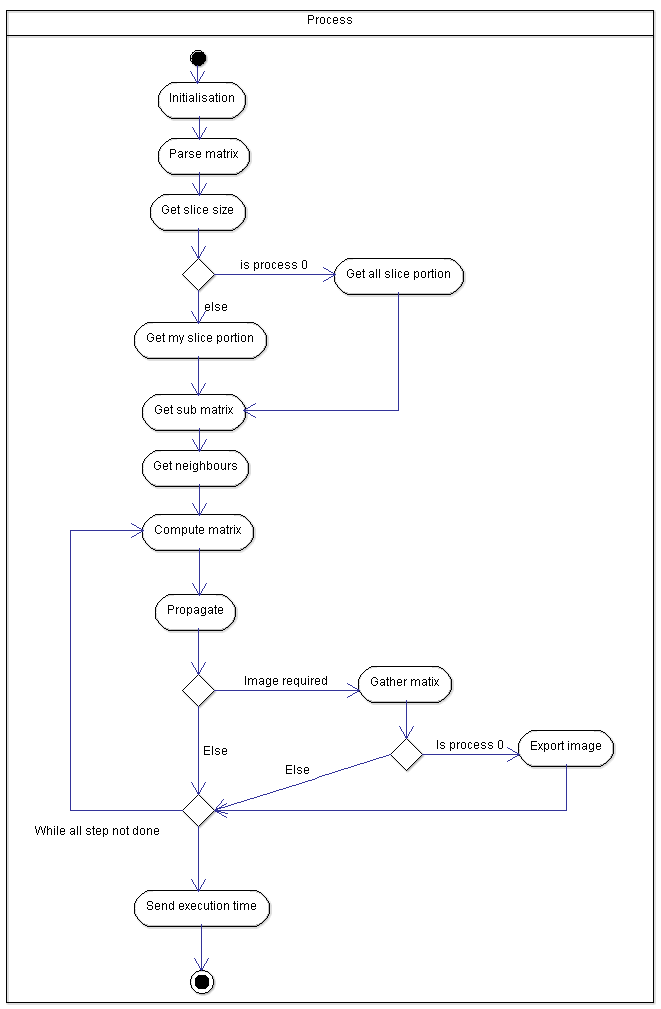
\includegraphics[scale=0.8]{activity.png}
		\caption{Activity diagram}
		\label{Activity diagram}
	\end{figure}
\end{center}

\section{Algorithm}
\subsection{Get slice size}
With a number N, a width x and a height y, the output is two number a and b such that a*b = N\\
First, a is set to be the floor of the root of N, then N is divide by a and while the result of the division is not an integer a is decreased.\\
After that, b is N/a.\\
All the possible result are saved in an array and then the algorithm select the one which have the ratio a/b closest to x/y.\\
The last step will divide the matrix in rectangle with the height and the width as equal as possible in order to have the smallest perimeter and therefore the least neighbours.
\subsection{Get slice portion}
With a matrix size, two numbers, x and y, which makes a division of the matrix, and which portion is required, defined by two number a and b, the result should be two cells position, the portion is the square between these two.\\
First, the algorithm calculate the width and the height of the portion by dividing the size of the width and the height of the matrix by x and y respectively, it saves the eventual rest.\\
The top left cell of the portion is (a*x, b*y) then it must adjust the result if there is a rest.\\
If a is bigger or equal than the width rest then the a*x is increased by this restl, in order to translate the portion. If a is smaller than the width rest then the width position of the first cell is translated by a because it means that a previous portion were taking one extra row.\\
The same process is used to adjust the height of the cell.\\
The last cell is the first plus the size of a portion, and if the rest was not handle by the previous portions, the current portion is increased by one.
\subsection{Get neighbours}
Each worker have eight neighbours, who can be themselves. To retrieve them, the first thing to do is to get his position x, y in the divided matrix from his process number. The x position is the process ID divided by the number of portion on the width of the matrix and y is the rest of that division.\\
Then the x, y  position of the neighbours can be easily found and the process id of the neighbours are found by multiplying x by the number of portion on the width of the matrix and adding y.

\section{Difficulties meet}
\subsection{Dividing the matrix}
The way the matrix is divided is explained in the Algorithm section, the resulting portion does not always have the same size. If the width of the matrix is 11 and there is 3 portion, the width of the portions wouldl be 4, 4 and 3. The problem is that the implementation use common message such as gather, so every process have to send the same number of message. During the process of the generation of the image, all process send their computable matrix to the master, all the process are in a double loop to cover the whole matrix but they cannot use the size of their computable matrix, they must use the size of the biggest computable matrix which is the matrix of the process 0 (it will always be) so the process 0 will broadcast the size of its portion and all the other process will run through their matrix using these sizes and if the  matrix is smaller, the process will send an impossible value (2 in the implementation), the master who gather the information will discard all the value if it is 2.
\subsection{Number of process}
There is one case where the number of process might be a problem, here is an example : the height of the matrix is 27 and the width is 5, if the number of process is 29, the slicing of the matrix will be 29*1 because 29 is a prime number but it is not possible to divide the number of lines in 29 because there is only 27. If this happens, in other words, if the number of portion on the height of the matrix is bigger than the number of line of the matrix then one process is discarded and the slice size is recalculated, in the example there would be 28 process which can be divided in 2*14.
\subsection{Protocol}
In the first implementation of the protocol two parts were different. First the master would him only parse the matrix and then send it on the network, I later found that it was way faster for each process to parse it itself.\\
The second difference is that after the computation each worker would send his computable matrix to the master and the master would reform the whole matrix and then resend to each process their neighbour matrix. The number of communication was really bigger than the new protocol where the process only communicate with their neighbours and they send only useful information, only the perimeter of their computable matrix.

\section{Conclusion}
The main difficulty of the project was to implement it on several process.\\
In order to improve the performance of the project, the number of communication between the process must be as small as possible. To do so, two main choice were done. First the process communicate only with their neighbours to avoid unnecessary message (except when an output is required) and secondly the portions for each worker are as squared as possible to have the smallest perimeter possible an therefore the fewest neighbours.\\
To discuss the result of the application, it is clear that the execution time is not always decreasing with the number of process. The execution time can be divided in two, the computing time and the communication time, the more process there is, the smaller the computing time but the bigger the communication time. The best number of process will be the one where the sum of the computing time and the communication time is minimal.

\end{document} 